\chapter{Regulator rozmyty dla modelu helikoptera}
\section{Wstęp}
Celem przedstawionych w niniejszym rozdziale badań było sprawdzenie jak regulator rozmyty współpracuje z rzeczywistym obiektem. Do eksperymentów wykorzystany został model helikoptera oraz jego model matematyczny sporządzony na potrzeby Laboratorium Problemowego. Zadaniem zaprojektowanego regulatora była stabilizacja układu w zadanym położeniu w osi poziomej.

\section{Model matematyczny}
Obiekt opisany jest następującymi równaniami:
\begin{equation}
\begin{aligned}
J_v \frac{d^2\alpha_v}{dt^2} &= -f_v\frac{d\alpha_v}{dt}+a\cdot sin(\alpha_v-\alpha_{v0})+M_v(\omega_v)\\
I_v\frac{d\omega_v}{dt} &= u_v - H_v^{-1}(\omega_v)
\end{aligned}
\label{eq:model_vertical1}
\end{equation}
\noindent gdzie:\newline
\(\alpha_v\) jest kątem obrotu w płaszczyźnie pionowej,\newline
\(J_v\) jest momentem bezwładności względem osi obrotu w płaszczyźnie pionowej,\newline
\(f_v\) jest współczynnikiem tarcia lepkiego,\newline
\(a\) jest momentem sił grawitacji,\newline
\(\alpha_{v0}\) jest kątem równowagi układu w płaszczyźnie pionowej,\newline
\(I_v\) jest momentem bezwładności dużego śmigła,\newline
\(H_v^{-1}(\omega_v)\) jest charakterystyką statyczną układu silnik-śmigło dla silnika głównego,\newline
\(\omega_v\) jest prędkością obrotową silnika głównego,\newline
\(M_v(\omega_v)\) jest momentem sił generowanym przez silnik główny,\newline
\(u_v\) jest współczynnikiem wypełniania sygnału PWM dla silnika głównego.\\\\
%
Równania stanu sporządzone na podstawie równań \ref{eq:model_vertical1} mają postać:
\begin{equation}
\begin{aligned}
\dot x_1 &= x_2\\
\dot x_2 &= -\frac{f_v}{J_v}x_2+\frac{a}{J_v}\sin (\alpha_v-\alpha_{v0})+\frac{M_v(\omega_v)}{J_v}\\
\dot x_3 &= \frac{u_v}{I_v}-\frac{H_v^{-1}(\omega_v)}{I_v}
\end{aligned}
\label{eq:ss_vertical1}
\end{equation}
%
Proces identyfikacji parametrów równań \ref{eq:ss_vertical1} opisany jest w pracy \cite{LP}.

\section{Regulator referencyjny}
Aby dobrać strukturę regulatora rozmytego typu Sageno podjęto decyzję o wykorzystaniu regulatora LQI. Podejście to wymagało zlinearyzowania równań \ref{eq:ss_vertical1} oraz zaprojektowania obserwatora Luengergera (\cite{LP}) w celu estymacji pełnego stanu obiektu.\\ 
Zlinearyzowany model w położeniu poziomym opisany jest równaniem 
\begin{equation}\label{key}
\begin{aligned}
\dot x = Ax + B \\
y = Cx + D
\end{aligned}
\end{equation}
gdzie:
\begin{equation}
\begin{aligned}
A &=
\begin{bmatrix}
0 & 1 & 0\\
-4.4005 & -0.0695 & 0.0244\\
0 & 0 & -2.8870
\end{bmatrix}\\
B &=
\begin{bmatrix}
0\\
0\\
577.5771
\end{bmatrix}\\
C &=
\begin{bmatrix}
1 & 0 & 0
\end{bmatrix}\\
D &= 0
\end{aligned}
\end{equation} 
Przyjęto następujące wartości własne obserwatora:
\begin{equation}
\begin{aligned}
\lambda_1 &= -3\\
\lambda_2 &= -6\\
\lambda_3 &= -9
\end{aligned}
\end{equation}
Obserwator Luenbergera pełnego rzędu opisany jest równaniem różniczkowym
\begin{equation}
\dot w = Aw+L(y-Cw)+Bu
\end{equation}
\noindent gdzie:\newline
\(A\) jest macierzą stanu obserwowanego układu,\newline
\(B\) jest macierzą sterowania obserwowanego układu,\newline
\(C\) jest macierzą wyjścia obserwowanego układu,\newline
\(G\) jest macierzą wybraną tak, by wartości własne macierzy \(A-LC\) miały ujemne części rzeczywiste,\newline
\(w\) estymuje obserwowany stan.
\paragraph*{}
Wybrana macierz \(L\) miała następującą postać:
\begin{equation}
L =
\begin{bmatrix}
15.0434\\
49.9218\\
87.9693
\end{bmatrix}
\end{equation}
%
Regulator LQI opisany jest zależnością 
\begin{equation}
\begin{aligned}
J&=\int\limits_0^{\infty}(x^TQx+u^TRu)dt\\
Q&=\begin{bmatrix}
10 & 0 & 0 & 0\\
0 & 0 & 0 & 0\\
0 & 0 & 0 & 0\\
0 & 0 & 0 & 1
\end{bmatrix}\\
R&=1
\end{aligned}
\end{equation}
\noindent gdzie:\newline
\(x_4\) jest całką z uchybu kąta.\\\\
%
Wektor wzmocnień \ref{wzmocnienieLQI} regulatora został wyliczony za pomocą funkcji \textit{lqi} środowiska \textit{Matlab}.
\begin{equation}
K=\begin{bmatrix}
0.3154 & 0.7105 & 0.0042 & -1
\end{bmatrix}
\label{wzmocnienieLQI}
\end{equation}

\section{Regulator rozmyty}
Do doboru struktury regulatora rozmytego typu Sageno wykorzystano funkcję\textit{genfis} środowiska \textit{Matlab}. W pierwszym etapie sprawdzono jakość regulacji projektując regulator \textit{fuzzy} na bazie modelu matematycznego. Na rysunku  \ref{por_model_lqi_fuzzy} przedstawiono odpowiedzi modelu obiektu w przypadku działania regulatora LQI i fuzzy.\\
%
\begin{table}[h]
	\caption{Porównanie wska\'zników jakości regulator LQI i fuzzy dla modelu.}
	\label{por_reg_lqi_fuzz_model}
	\centering
	
	\begin{tabular}{|c|M{2.5cm}|M{2.5cm}|M{2.5cm}|}
		\hline
		Regulator &$J_1$\\
		\hline
		LQI &0.102\\
		\hline
		fuzzy & 0.102\\
		\hline
	\end{tabular}
\end{table}
\FloatBarrier
Wartości wska\'zników jakości zaprezentowane w tabeli \ref{por_reg_lqi_fuzz_model} oraz przebiegi zaprezentowane na rysunkach \ref{por_model_lqi_fuzzy} i \ref{diff_model_lqi_fuzzy} pokazują że w przypadku matematycznego modelu rozważanego obiektu klasyczny regulator LQI może być z powodzeniem zastąpiony regulatorem rozmytym bez pogorszenia jakości sterowania.

 \begin{figure}[h!]
	\noindent\makebox[\textwidth]{
		\centering
		\subfloat[][Porównanie działania regulatora LQI i fuzzy.]{
			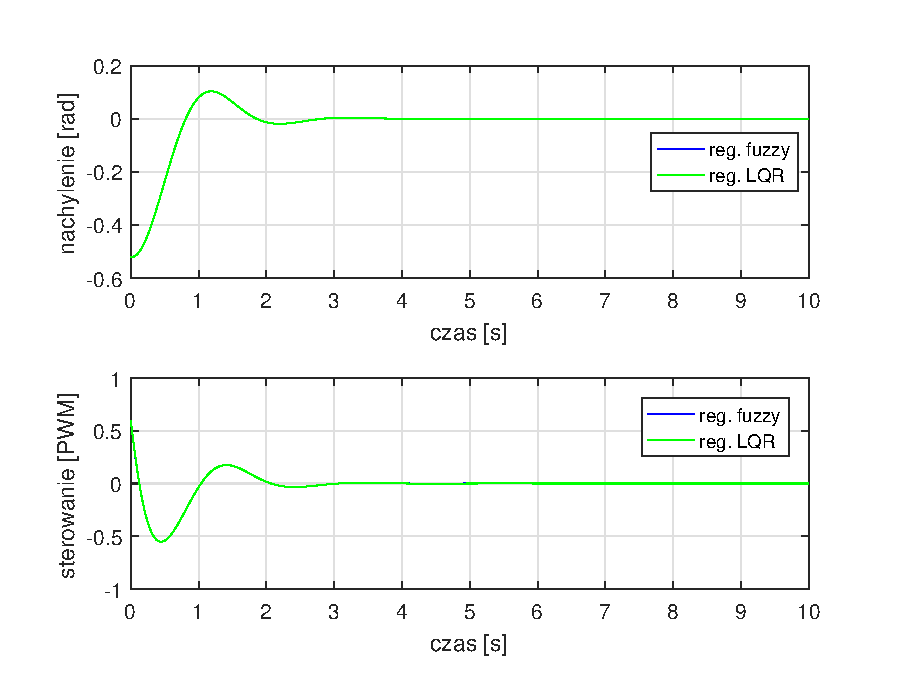
\includegraphics[scale=0.65]{fig/por_fuzzy_model_lqi.eps}
			\label{por_model_lqi_fuzzy}
		}
		\hfill
		%\begin{figure}[h!]
		%	\centering
		\subfloat[][Różnica działania regulatora LQI i fuzzy.]{
			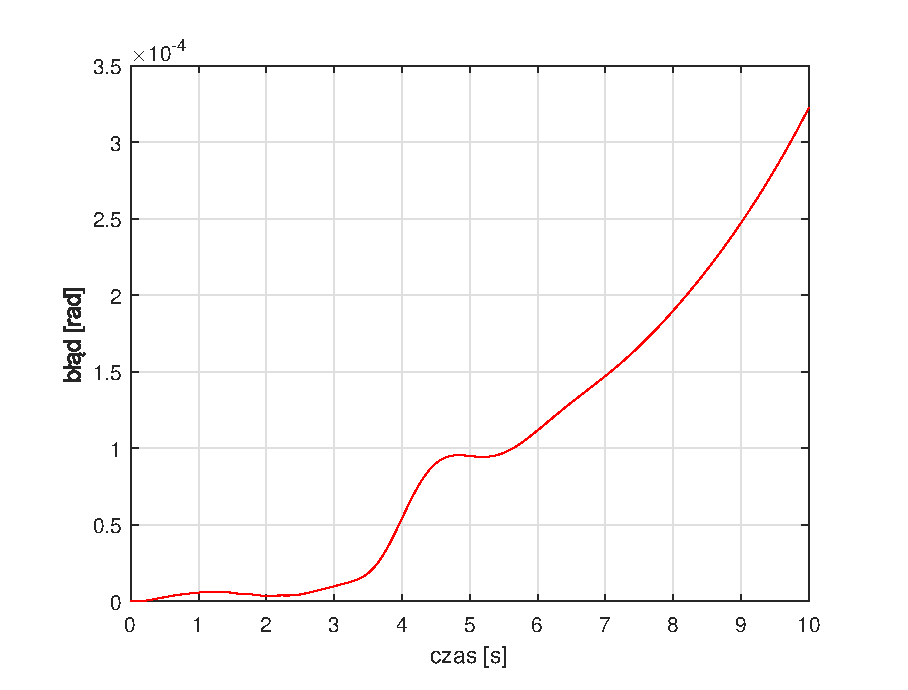
\includegraphics[scale=0.65]{fig/diff_fuzzy_model_lqi.eps}
			\label{diff_model_lqi_fuzzy}
		}
		
		%{a) Porównanie wyjścia obiektu i estymaty. b) Porównanie błędów wyjścia i estymaty.}
	}
	\caption{Działanie regulatora dla modelu obiektu.}		
\end{figure}


%\begin{figure}[h!]
%	\centering
%	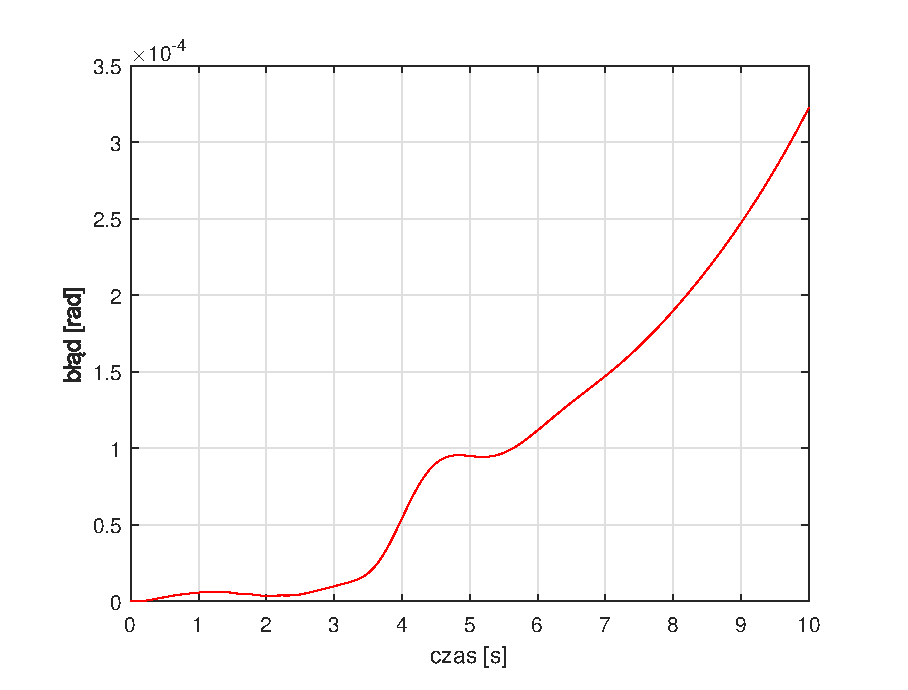
\includegraphics[scale = 0.8]{fig/diff_fuzzy_model_lqi}
%	\caption		
%	{Różnica działania regulatora LQI i fuzzy.}
%	\label{diff_model_lqi_fuzzy}
%\end{figure} 

\begin{figure}[h!]
	\centering
	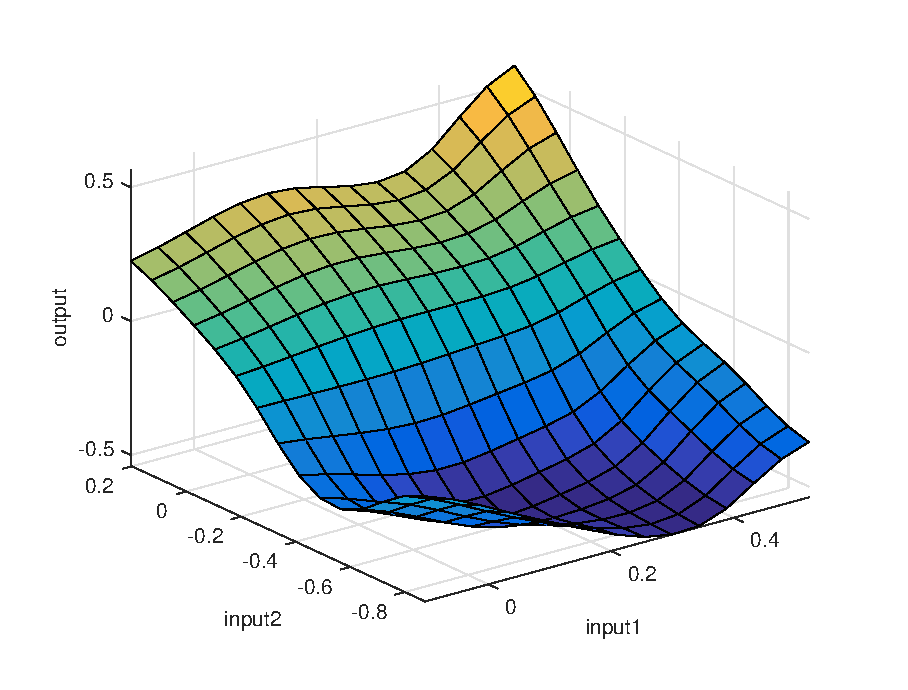
\includegraphics[scale = 0.8]{fig/fuzzy_hel_model_surf.eps}
	\caption		
	{Powierzchnia sterowania dla modelu obiektu rzutowana na pierwszą i drugą zmienną stanu.}
	\label{fuzzy_hel_model_surf}
\end{figure} 
\FloatBarrier
Następnie postanowiono sprawdzić działanie regulatora na rzeczywistym obiekcie. W tym celu na wejście obiektu podano sygnał pokazany na rysunku \ref{stan_obiekt}. Podczas działania układu rejestrowano wartości zmiennych stanu (wyjście z obserwatora Luenbergera), całki uchybu regulacji oraz sterowania.\\
Zdecydowano, że do procedury \textit{genfis} podane zostaną przebiegi zarejestrowanych zmiennych pomiędzy 20 a 40 sekundą. Decyzja ta wynikała z chęci uniknięcia optymalizacji struktury regulatora na danych z początkowego etapu działania obserwatora gdy estymowane wartości zmiennych stanu znacznie odbiegały od rzeczywistych. \\
Niestety nie udało się przetestować działania tak zaprojektowanego regulatora na obiekcie ponieważ \textit{Simulink} nie potrafił uruchomić modelu w czasie rzeczywistym gdy był wykorzystywany w nim bloczek  \textit{Fuzzy Logic Controller}. \\
 \begin{figure}[h]
	\noindent\makebox[\textwidth]{
		\centering
		\subfloat[][Przebieg zmiennych stanu.]{
			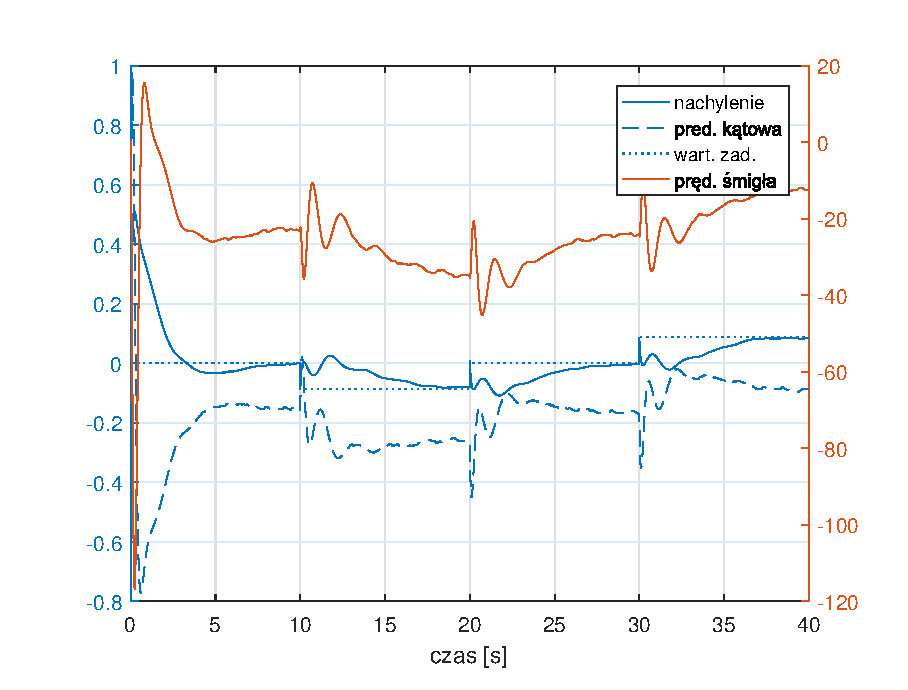
\includegraphics[scale=0.65]{fig/stan_obiekt.eps}
			\label{stan_obiekt}
		}
		\hfill
		%\begin{figure}[h!]
		%	\centering
		\subfloat[][Sterowanie podawane na obiekt.]{
			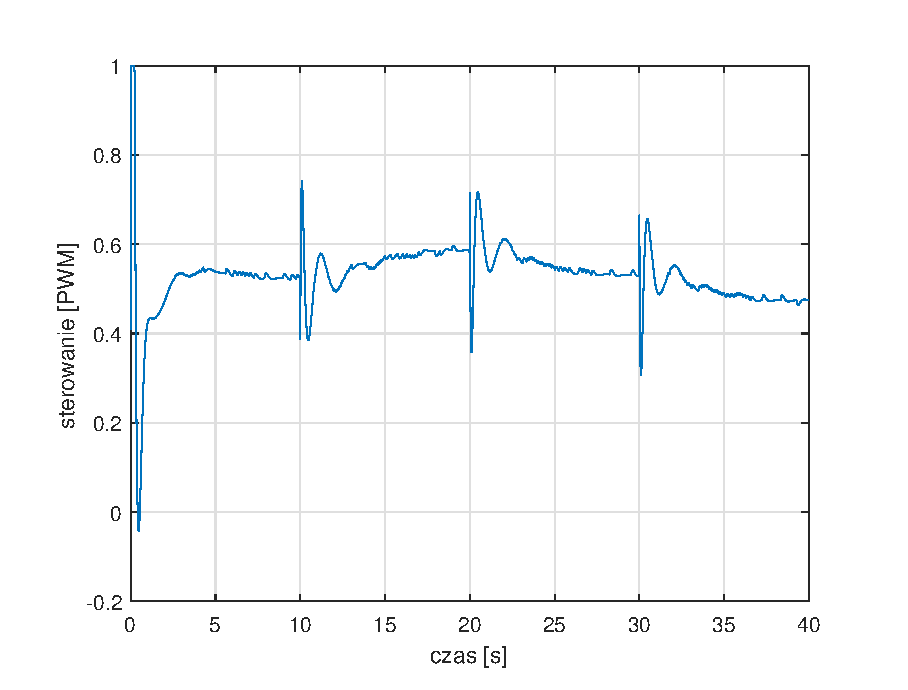
\includegraphics[scale=0.65]{fig/ster_obiekt.eps}
			\label{ster_obiekt}
		}
		
		%{a) Porównanie wyjścia obiektu i estymaty. b) Porównanie błędów wyjścia i estymaty.}
	}
	\caption{Dane wykorzystane do optymalizacji struktury reg. rozmytego.}		
\end{figure}
%
\begin{figure}[h]
	\centering
	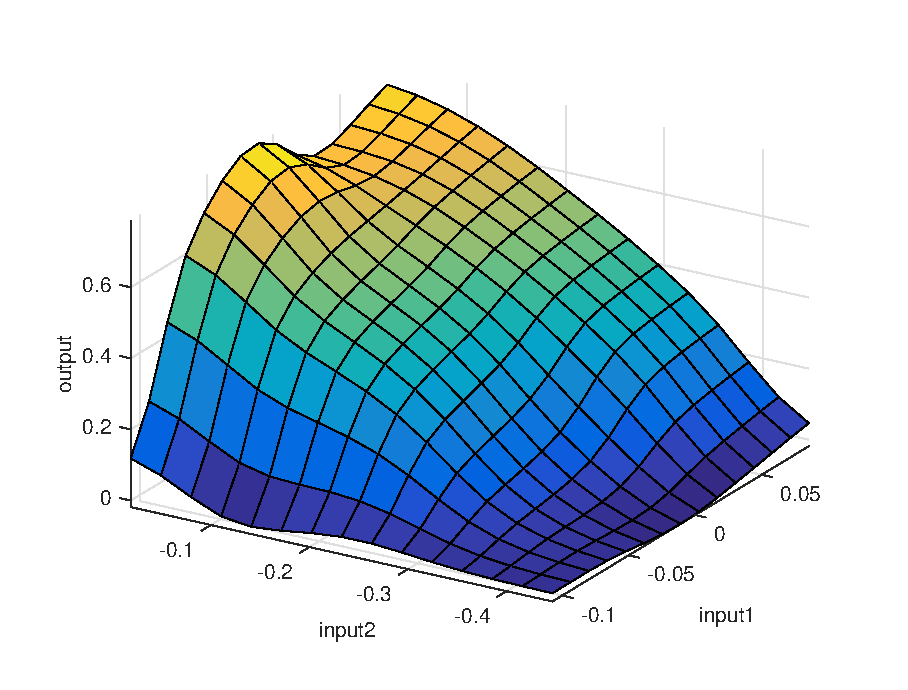
\includegraphics[scale = 0.8]{fig/fuzzy_obiekt_surf.eps}
	\caption		
	{Powierzchnia sterowania dla obiektu rzutowana na pierwszą i drugą zmienną stanu.}
	\label{fuzzy_hel_obiekt_surf}
\end{figure} 
\begin{figure}[h]
	\centering
	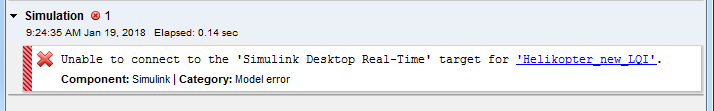
\includegraphics[scale = 0.8]{fig/bladSim.PNG}
	\caption		
	{Błąd zwracany przez \textit{Simulink}.}
	\label{bladSim}
\end{figure} 
\FloatBarrier
 Na podstawie powierzchni sterowania zaprezentowanej na rysunku \ref{fuzzy_hel_obiekt_surf} można stwierdzić że struktura regulatora jest podobna do struktury uzyskanej na podstawie danych symulacyjnych (rysunek \ref{fuzzy_hel_model_surf}). 
 